\chapter{Implementation}

\section{Vivado HLS}

Listing~\ref{lst:convolution_engine_vivado_hls} shows the convolution engine design which would convolve a 1024$\times$1024 image with a
3$\times$3 kernel. This is a functionally correct but an unoptimized design for the convolution engine of this size.

\singlespacing
\scriptsize
\begin{lstlisting}[language=C++, caption=Core Vivado HLS, label={lst:convolution_engine_vivado_hls}]
#include "ap_int.h"
#include "hls_stream.h"

void core(char* init_row, char* kernel_data_row, char* row_dest) {
    #pragma HLS INTERFACE s_axilite port=return
    #pragma HLS INTERFACE m_axi port=init_row offset=slave
    #pragma HLS INTERFACE m_axi port=kernel_data_row offset=slave
    #pragma HLS INTERFACE m_axi port=row_dest offset=slave

    // assume an image size of 3x3 for now and the image is already padded with zeros.
    // assuming a kernel of size 3x3 which is symmetric or already flipped stored at 
    // the kernel storage location.

    // init_row points to a 5x5 image matrix in hardware.

    char i,j;
    char index=0;
    char acc=0;
    char rows = 3; 
    char cols = 3;

    for(i=0;i<rows;i+=rows)
    {
	for(j=0;j<cols;j++)
	{
		acc+= kernel_data_row[0]*(*(init_row+i+j));
		acc+= kernel_data_row[1]*(*(init_row+i+j+1));
		acc+= kernel_data_row[2]*(*(init_row+i+j+2));
		acc+= kernel_data_row[3]*(*(init_row+i+rows+j));
		acc+= kernel_data_row[4]*(*(init_row+i+rows+j+1));
		acc+= kernel_data_row[5]*(*(init_row+i+rows+j+2));
		acc+= kernel_data_row[6]*(*(init_row+i+2*rows+j));
		acc+= kernel_data_row[7]*(*(init_row+i+2*rows+j+1));
		acc+= kernel_data_row[8]*(*(init_row+i+2*rows+j+2));
		row_dest[index] = acc;
		index++;
	}
    }
}
\end{lstlisting}
\normalsize
\doublespacing


\section{AHIR HLS}

\subsection{C to VHDL}

\begin{figure}[H]
\centering
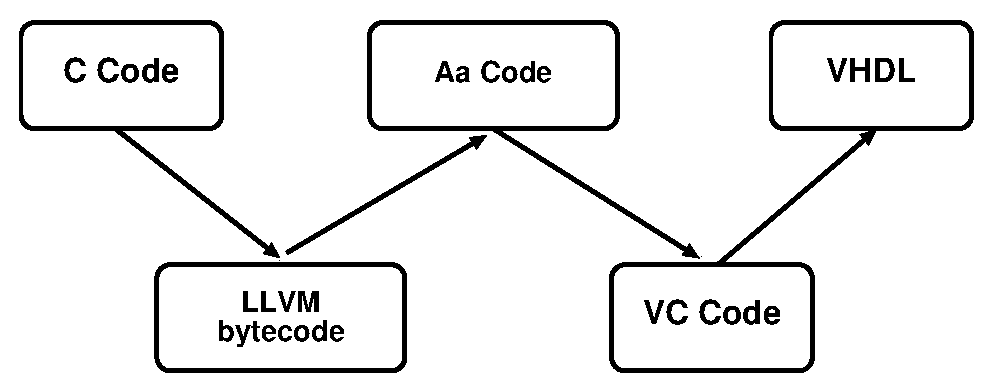
\includegraphics[width=\textwidth]{eps_pdf_sources/convolution_engine/implementation/c_2_vhdl}
\caption{C to VHDL design flow}
\label{c2vhdl}
\end{figure}

\begin{flushleft}
\textit{VC} : Virtual circuit format\\
\textit{Aa} : Aa language format(explained below)
\end{flushleft}

\subsection{Aa to VHDL}

Aa is a programming language for the description of algorithms, with the ultimate aim being the conversion of these algorithms into a
hardware implementation. The control-flow in an Aa program corresponds to a petri net of a specific class. The data-flow is constructed
using static single-assignment variables (which can be assigned to only once), storage objects, messaging pipes and constants. Pointers to
storage objects can be created and manipulated (pointer arithmetic, dereferencing etc.) in the usual way. A program in Aa can also be
viewed as a description of a system which reacts with its environment through input and output ports. Thus, an Aa program can either be
executed on a computer, or be mapped to a logic circuit. 

\begin{figure}[H]
\centering
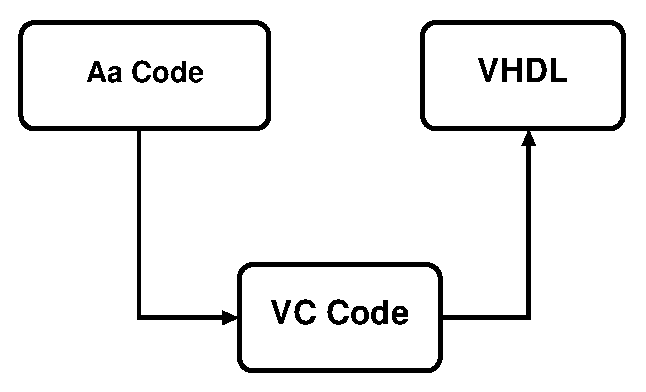
\includegraphics[width=0.8\textwidth]{eps_pdf_sources/convolution_engine/implementation/aa_2_vhdl}
\caption{Aa to VHDL design flow}
\label{aa2vhdl}
\end{figure}

\section{Testing Setup}

\subsection{AHIR Testbenches}

\subsubsection{Software Test}
%\paragraph{testbench\_sw \\}
This method of testing the design works only for the C to VHDL design flow. We have a common C testbench file between software and hardware
testing. This testbench when compiled for software testing runs different system units as multiple threads which communicate through
software pipes.

\subsubsection{Hardware Test}
%\paragraph{testbench\_hw and ahir\_system\_test\_bench \\}
This method of testing the design works for the C to VHDL design flow as well as Aa to VHDL design flow. We have a common C testbench file
between software and hardware testing. This testbench when compiled for hardware testing generates to two executables named
\verb|testbench_hw| and \verb|ahir_system_test_bench| which can be run in different shells one after another to start a ghdl simulation
enabled by communicating through sockets.
